\subsection{Kiểm thử từng thành phần}

\begin{frame}[t,fragile]
\frametitle{Kiểm thử Module 4G/GPS \& Khởi tạo hệ thống}
\begin{columns}[T]
    %----------------- Column Log -----------------%
    \column{0.55\textwidth}
    \begin{minted}[fontsize=\scriptsize,breaklines]{text}
I (2329)  SIM_4G: Received: Quectel EG800K
OK
I (5329)  SIM_4G: Received: +CSQ: 31,99
OK
I (28339) SIM_4G: Received: +QIACT: 1,1,1,"9.204.251.200"
OK
I (34349) SIM_4G: Received: +QGPSLOC: 10.88862,106.77975
OK
I (9961)  SIM4G_AT: Initializing SIM4G AT driver...
I (10011) APP_MAIN: System initialization complete.
I (10021) APP_MAIN: Application started successfully
    \end{minted}

    %----------------- Column Phân tích -----------------%
    \column{0.45\textwidth}
    \begin{itemize}
        \item \textbf{Mục đích:} 
        \begin{itemize}
            \item Xác nhận giao tiếp AT command, kết nối 4G và thu nhận GPS.
            \item Kiểm tra các module SIM4G-GPS, Wi-Fi và các tác vụ chính.
        \end{itemize}
        \item \textbf{Quy trình:}
        \begin{enumerate}
            \item Khởi tạo UART, kiểm tra modem và SIM.
            \item Đánh giá chất lượng sóng (\texttt{+CSQ}).
            \item Cấu hình APN, kích hoạt PDP context.
            \item Bật GPS và truy vấn tọa độ.
        \end{enumerate}
        \item \textbf{Kết luận:} 
        \begin{itemize}
            \item Module 4G/GPS hoạt động ổn định, sẵn sàng gửi cảnh báo và thông tin định vị.
            \item Hệ thống khởi tạo thành công, tích hợp phần mềm và phần cứng ổn định.
        \end{itemize}
    \end{itemize}
\end{columns}
\end{frame}
% ----------------------------
% Slide: Kiểm thử MQTT
% ----------------------------
\begin{frame}[t,fragile]
\frametitle{Kiểm thử MQTT và truyền dữ liệu}
\begin{columns}[T]
    \column{0.55\textwidth}
    \begin{itemize}
        \item \textbf{Mục đích:} Kiểm tra kết nối broker MQTT và gửi bản tin định kỳ.
        \item \textbf{Log tiêu biểu:}
        \begin{minted}[fontsize=\footnotesize,breaklines]{text}
I (19961) USER_MQTT: MQTT_EVENT_CONNECTED
I (39991) JSON_WRAPPER: {"device_id":"ESP32_DEV_76E48B","fall_detected":false,...}
        \end{minted}
        \item \textbf{Kết luận:} Kết nối MQTT ổn định, dữ liệu được truyền tới hệ thống giám sát.
    \end{itemize}
    \column{0.45\textwidth}
    \begin{figure}
        \centering
        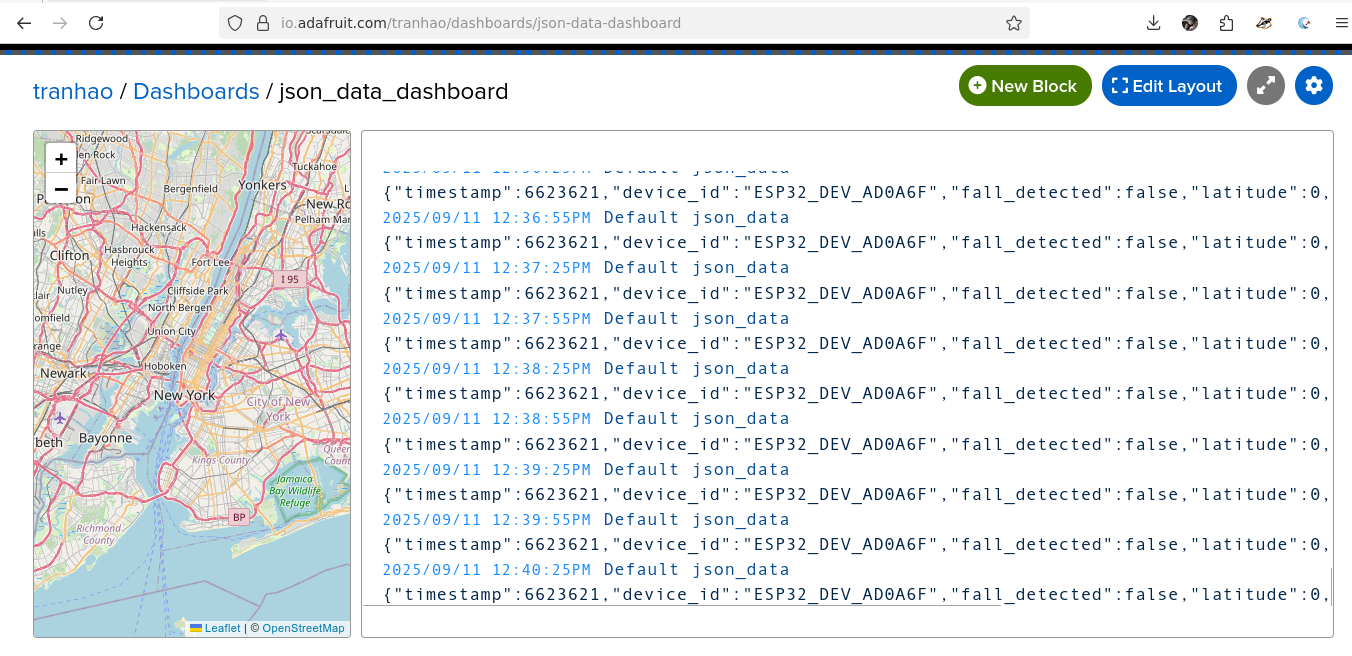
\includegraphics[width=0.75\linewidth]{json_data_dashboard.png}
        \caption{Dashboard hiển thị bản tin MQTT.}
    \end{figure}
\end{columns}
\end{frame}

% ----------------------------
% Slide: Phát hiện té ngã & cảnh báo
% ----------------------------
\begin{frame}[t,fragile]
\frametitle{Phát hiện Té ngã \& Xử lý Cảnh báo}
\begin{columns}[T]
    \column{0.55\textwidth}
    \begin{itemize}
        \item \textbf{Quy trình:}
        \begin{enumerate}
            \item Thuật toán ghi nhận chuỗi trạng thái \texttt{LOW\_G} $\to$ \texttt{HIGH\_G}.
            \item Kích hoạt cảnh báo: SMS, MQTT, buzzer, LED.
        \end{enumerate}
        \item \textbf{Log thực tế:}
        \begin{minted}[fontsize=\footnotesize,breaklines]{text}
\alert{E (159131) FALL_LOGIC: FALL DETECTED! Accel: 0.99 g}
I (159151) SIM4G_GPS: SMS request queued successfully
I (159881) SIM4G_AT: SMS sent successfully.
        \end{minted}
    \end{itemize}
    \column{0.45\textwidth}
    \begin{figure}
        \centering
        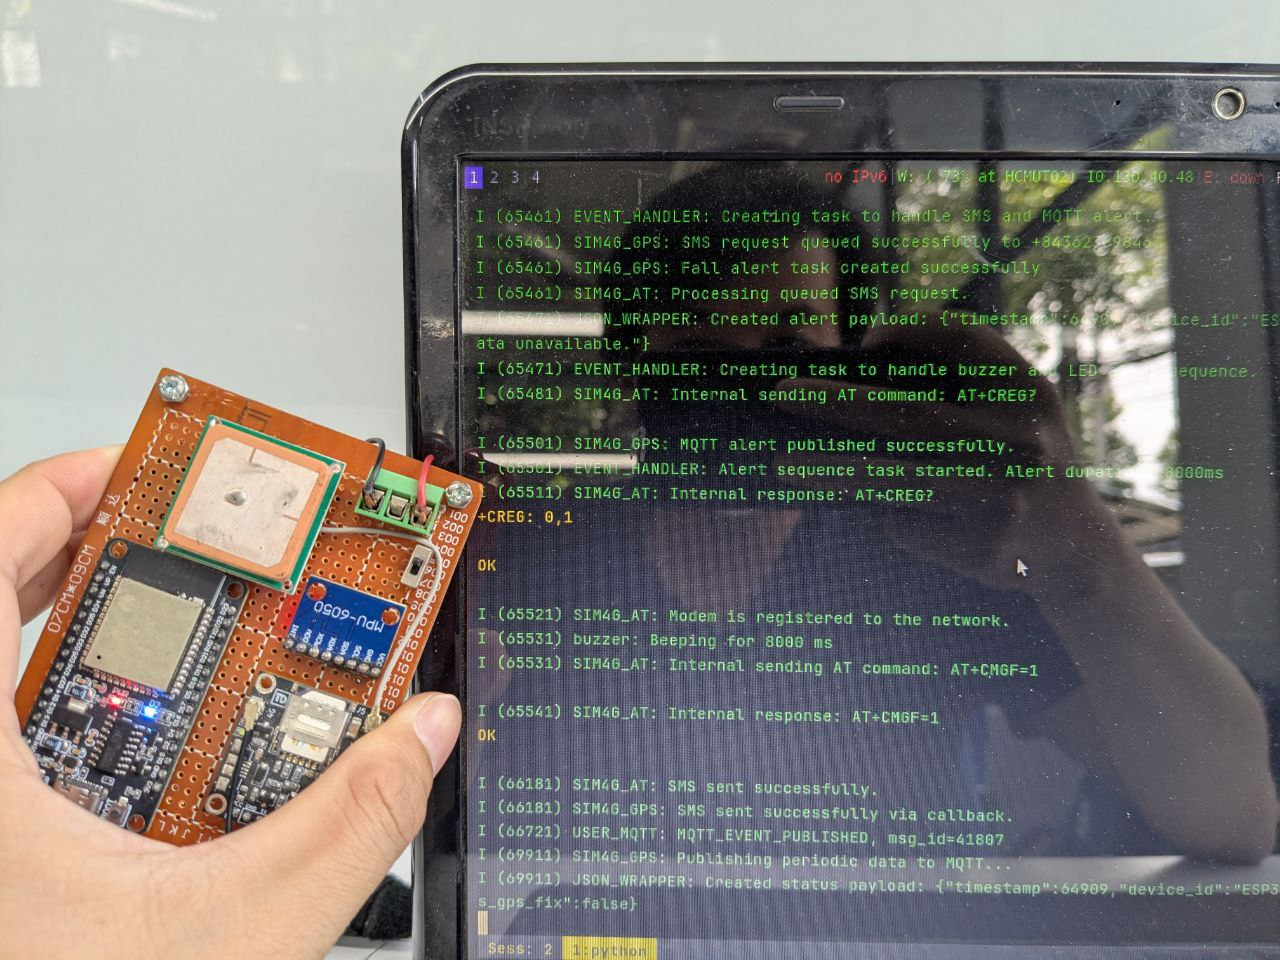
\includegraphics[width=0.75\linewidth]{module1_real_log.jpg}
        \caption{Log thực tế module cảm biến khi phát hiện té ngã.}
    \end{figure}
\end{columns}
\end{frame}

% ----------------------------
% Slide: Camera ESP32 – Luồng hình ảnh & nhận diện
% ----------------------------
\begin{frame}[t,fragile]
\frametitle{Camera ESP32-CAM: Luồng hình ảnh và xử lý}
\begin{columns}[T]
    %----------------- Column Hình -----------------%
    \column{0.55\textwidth}
    \begin{figure}[H]
        \centering
        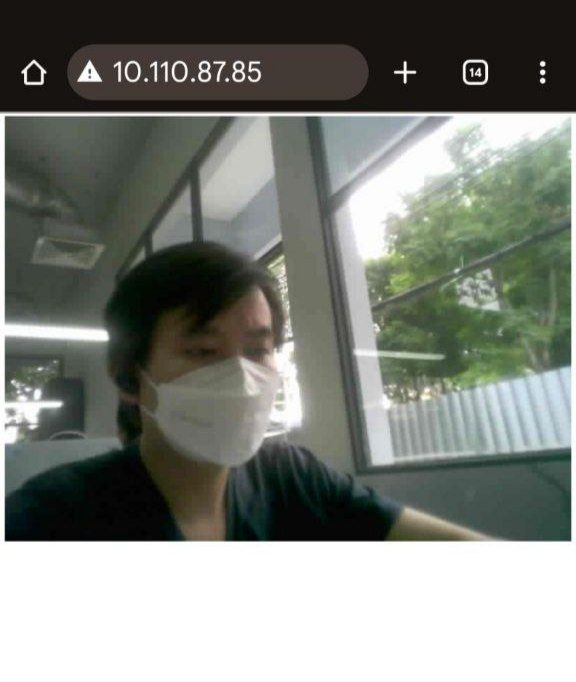
\includegraphics[width=\linewidth]{module2_stream_example.jpg}
        \caption{Luồng hình ảnh từ ESP32-CAM qua HTTP.}
    \end{figure}

    %----------------- Column Phân tích -----------------%
    \column{0.45\textwidth}
    \begin{itemize}
        \item \textbf{Mục đích:} Kiểm tra kết nối Wi-Fi và phát luồng hình ảnh.
        \item \textbf{Xử lý Python:}
        \begin{itemize}
            \item Nhận luồng video từ ESP32-CAM.
            \item Tiền xử lý khung hình.
            \item TensorFlow Lite phát hiện người, vẽ skeleton.
        \end{itemize}
        \item \textbf{Kết quả:} Thời gian thực 3–5 FPS, hoạt động ổn định.
        \item \textbf{Ứng dụng:} Cảnh báo té ngã, đồng bộ MQTT, gửi thông báo Telegram.
    \end{itemize}
\end{columns}
\end{frame}

% ----------------------------
% Slide: Xử lý nhận diện hình ảnh (Python)
% ----------------------------
\begin{frame}[t,fragile]
\frametitle{Xử lý nhận diện hình ảnh (Python)}
\begin{columns}[T]
    %----------------- Column Thông tin -----------------%
    \column{0.45\textwidth}
    \begin{itemize}
        \item \textbf{Mục đích:} Phát hiện người và trích xuất skeleton từ luồng video.
        \item \textbf{Quy trình:}
        \begin{itemize}
            \item Nhận luồng video từ ESP32-CAM.
            \item Tiền xử lý khung hình.
            \item TensorFlow Lite phát hiện người, vẽ skeleton.
        \end{itemize}
        \item \textbf{Kết quả:} Thời gian thực 3–5 FPS, hoạt động ổn định.
    \end{itemize}

    %----------------- Column Hình minh họa -----------------%
    \column{0.55\textwidth}
    \begin{figure}
        \centering
        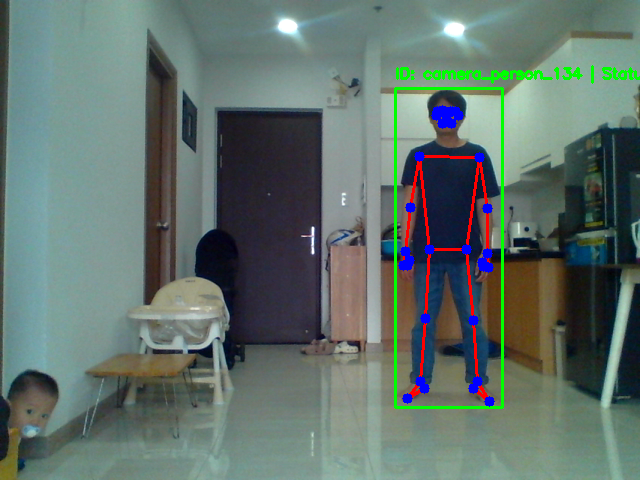
\includegraphics[width=\linewidth]{fall_detection_screen_shoot.png}
        \caption{Module Python phát hiện người và vẽ skeleton.}
    \end{figure}
\end{columns}
\end{frame}

% ----------------------------
% Slide: Log thực nghiệm Python
% ----------------------------
\begin{frame}[t,fragile]
\frametitle{Log Python}
\begin{columns}[T]
    %----------------- Column Log -----------------%
    \column{0.55\textwidth}
    \begin{minted}[fontsize=\scriptsize,breaklines]{text}
# Log Python xử lý luồng camera và điều phối cảnh báo
I (10521) PYTHON_APP: Frame received from ESP32-CAM
I (10535) PYTHON_APP: Preprocessing frame...
I (10612) PYTHON_APP: Person detected, skeleton extracted
I (10635) MQTT_CLIENT: Fall alert sent successfully
    \end{minted}

    %----------------- Column Kết luận -----------------%
    \column{0.45\textwidth}
    \begin{itemize}
        \item \textbf{Kết luận:} 
        \begin{itemize}
            \item Module Python hoạt động ổn định.
            \item Đồng bộ MQTT và kích hoạt cảnh báo thành công.
        \end{itemize}
        \item \textbf{Hình minh họa (tùy chọn):}
        \begin{figure}
            \centering
            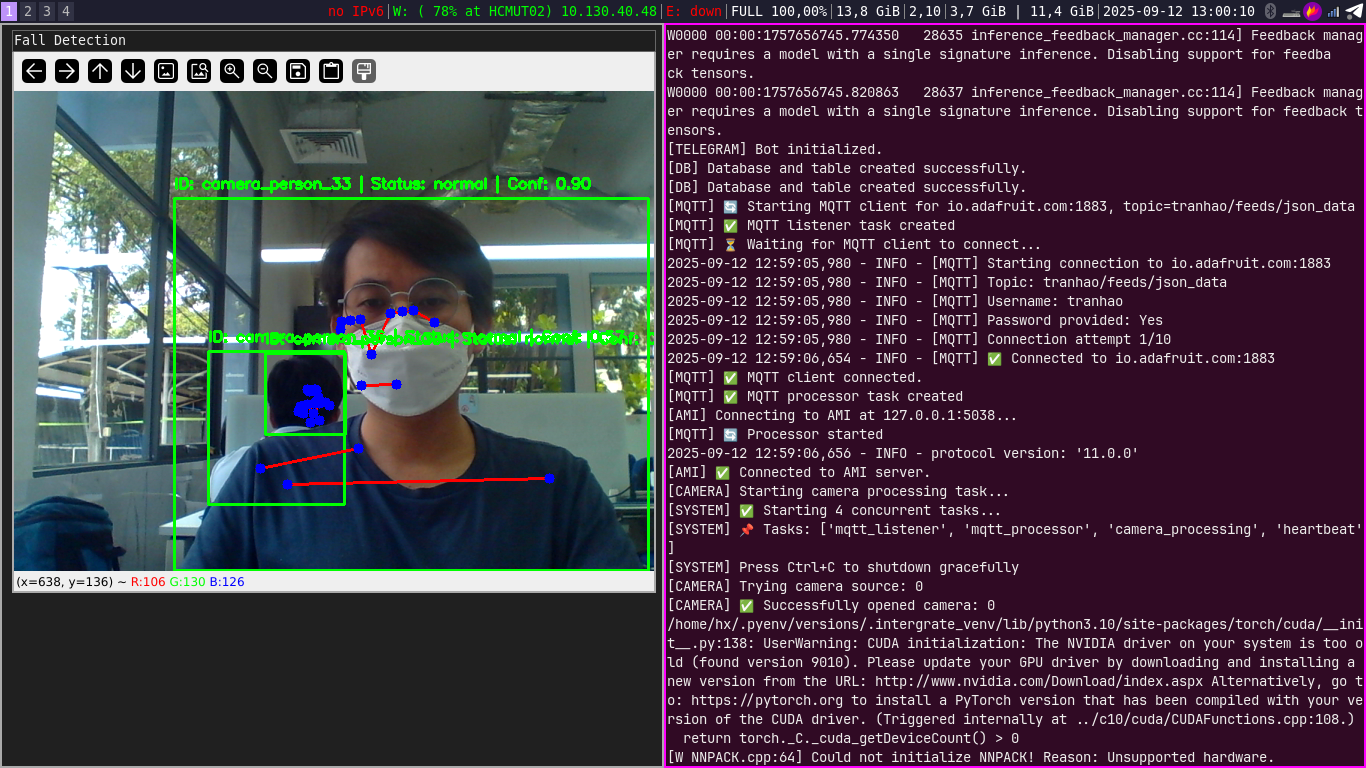
\includegraphics[width=\linewidth]{python_runing_log.png}
            \caption{Log Python xử lý luồng camera và cảnh báo.}
        \end{figure}
    \end{itemize}
\end{columns}
\end{frame}

% ----------------------------
%---- MPU6050------------
%----------------------------

\begin{frame}[t,fragile]
\frametitle{Đánh giá dữ liệu cảm biến (MPU6050) – Accel\_Mag}
\begin{columns}[T]
    %----------------- Column Hình -----------------%
    \column{0.55\textwidth}
    \begin{figure}[H]
        \centering
        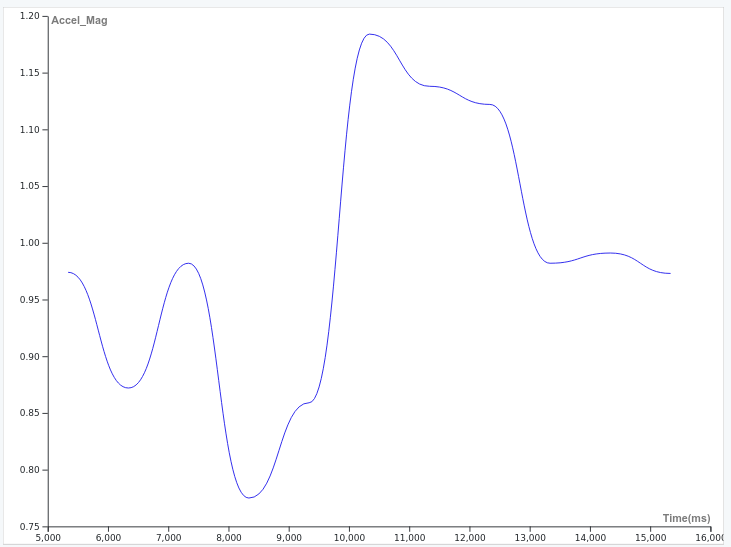
\includegraphics[width=\linewidth]{accel_time.png}
        \caption{Magnitude gia tốc (Accel\_Mag) theo thời gian. Xung lớn biểu thị té ngã.}
    \end{figure}

    %----------------- Column Thông tin -----------------%
    \column{0.45\textwidth}
    \begin{itemize}
        \item \textbf{Quy trình:} Giả lập té ngã, so sánh dữ liệu bình thường và té ngã.
        \item \textbf{Kết quả:}
        \begin{itemize}
            \item \textbf{Gyro (dps):} Bình thường $\approx \pm 1.5$; té ngã tăng $\approx \pm 250$.
            \item \textbf{Accel (g):} Bình thường $\approx 0.93$; té ngã $-2.0$ đến $+1.0$.
        \end{itemize}
        \item \textbf{Phân tích:}
        \begin{itemize}
            \item \textbf{Bình thường:} Gần 1\,g, dao động nhỏ.
            \item \textbf{Sự kiện té ngã:} Xuất hiện xung hoặc thay đổi đột ngột.
            \item \textbf{Hậu té:} Trở về gần 1\,g nhưng phân bố vector khác.
        \end{itemize}
        \item \textbf{Kết luận:} \textbf{Accel\_Mag} và \textbf{Gyro\_Mag} là chỉ báo hiệu quả để phát hiện té ngã.
    \end{itemize}
\end{columns}
\end{frame}

% ----------------------------
% Slide: Kiểm thử cảnh báo Telegram
% ----------------------------
\begin{frame}[t,fragile]
\frametitle{Kiểm thử cảnh báo qua Telegram}
\begin{itemize}
    \item \textbf{Cơ chế hoạt động:}
    \begin{itemize}
        \item \textbf{Phần cứng:} MQTT từ thiết bị -> trung tâm -> Telegram.
        \item \textbf{Python:} Camera -> Python gửi cảnh báo trực tiếp Telegram kèm hình.
    \end{itemize}
\end{itemize}
\end{frame}

% ----------------------------
% Slide: Thông báo Telegram
% ----------------------------
\begin{frame}[t,fragile]
\frametitle{Thông báo Telegram}
\begin{columns}[T]
    \column{0.4\textwidth}
    \begin{figure}[H]
        \centering
        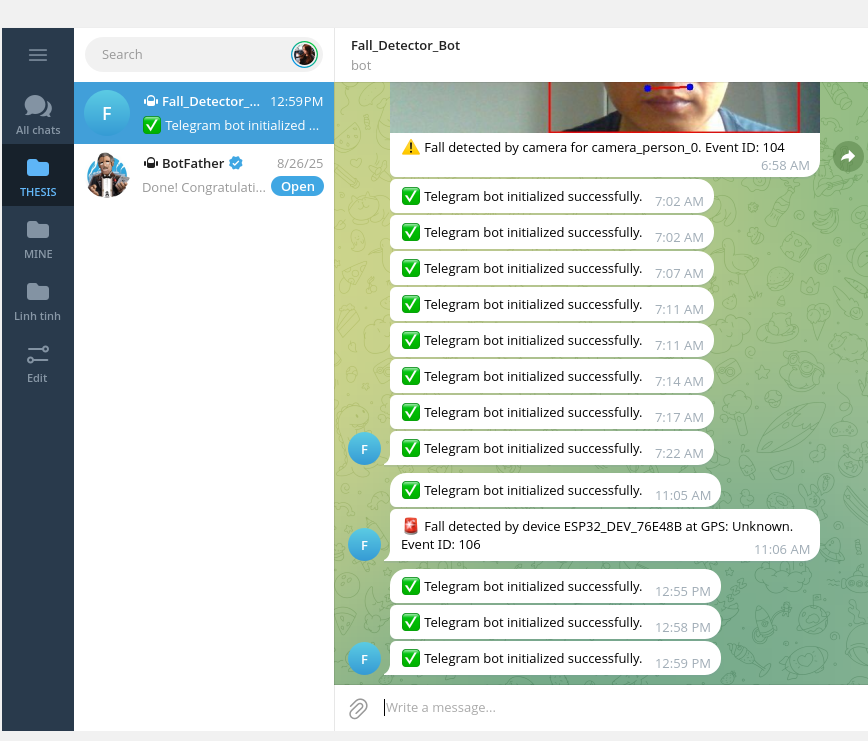
\includegraphics[width=0.70\linewidth]{telegram_fall_module1_send.png}
        \caption{Thông báo từ phần cứng.}
    \end{figure}
    \column{0.6\textwidth}
    \begin{figure}[H]
        \centering
        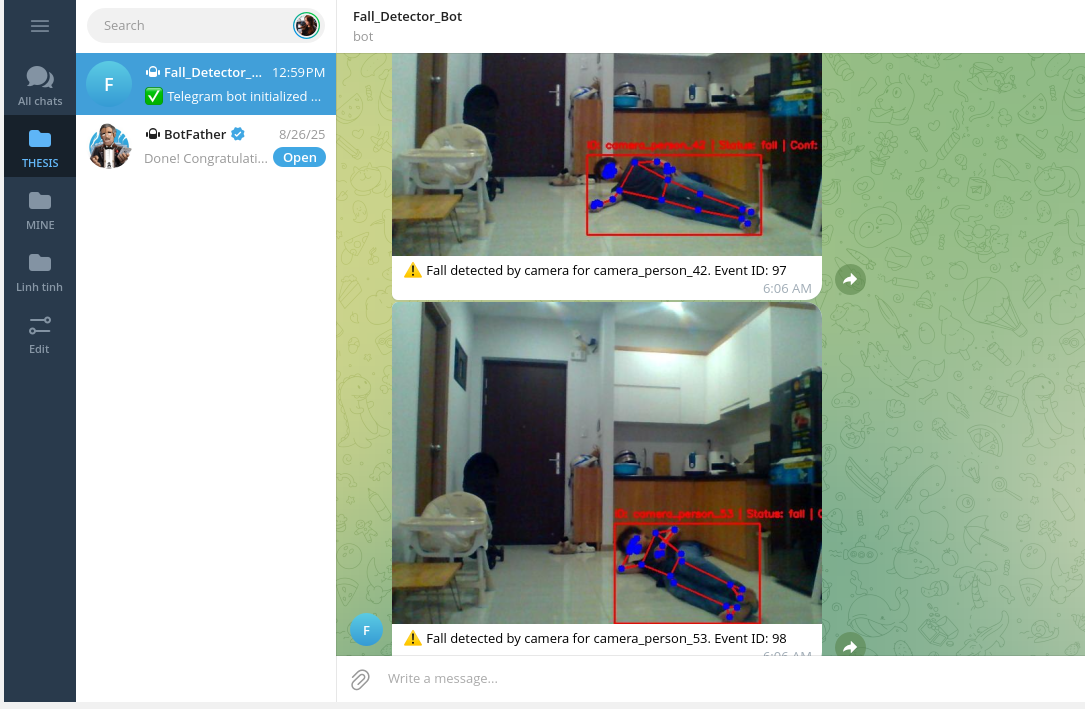
\includegraphics[width=0.70\linewidth]{telegram_python_fall_send.png}
        \caption{Thông báo từ Python.}
    \end{figure}
    \begin{itemize}
        \item \textbf{Kết luận:} Kênh Telegram hoạt động ổn định, đa nguồn cảnh báo tăng độ tin cậy.
    \end{itemize}
\end{columns}
\end{frame}
